

\tikzset{every picture/.style={line width=0.75pt}} %set default line width to 0.75pt        

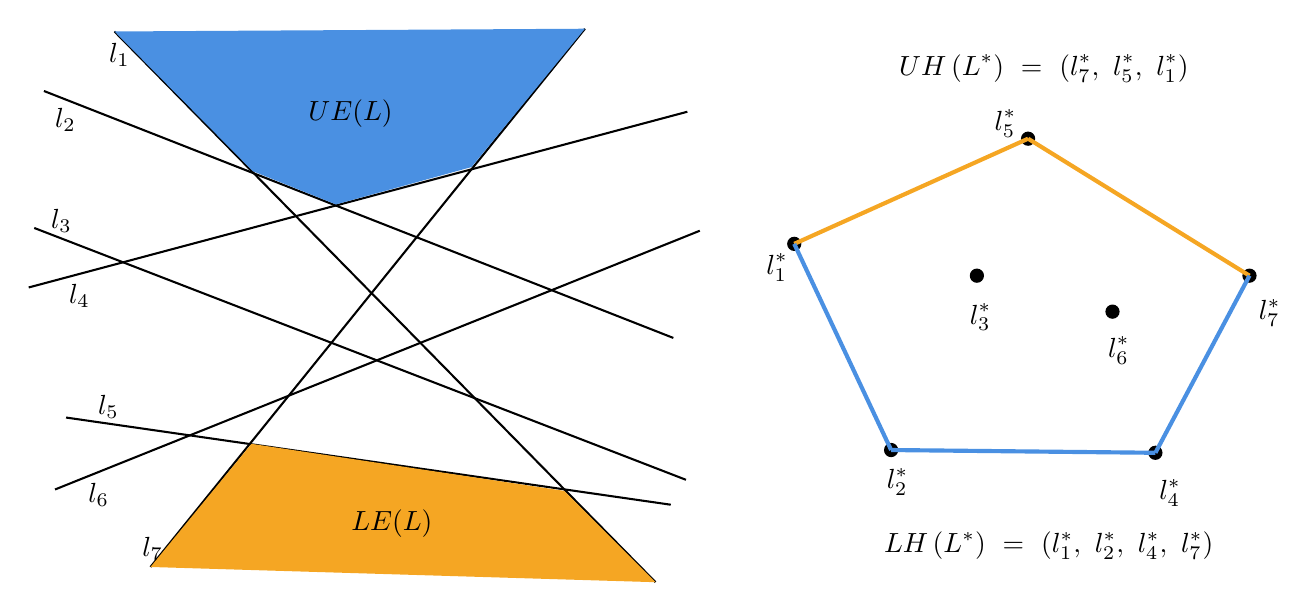
\begin{tikzpicture}[x=0.5pt,y=0.5pt,yscale=-1,xscale=1]
%uncomment if require: \path (0,420); %set diagram left start at 0, and has height of 420

%Straight Lines [id:da8861644180083026] 
\draw    (92.13,398.52) -- (406.13,9.52) ;
%Straight Lines [id:da40732713893670314] 
\draw    (457.13,409.52) -- (66.13,11.52) ;
%Straight Lines [id:da44367949821680464] 
\draw    (468.13,353.52) -- (31.13,290.52) ;
%Straight Lines [id:da2319769205561817] 
\draw    (470,233) -- (15.13,54.52) ;
%Straight Lines [id:da8632177571421473] 
\draw    (480.13,69.52) -- (4.13,196.52) ;
%Straight Lines [id:da43810226035482036] 
\draw    (489.13,155.52) -- (23.13,342.52) ;
%Straight Lines [id:da08264547138329514] 
\draw    (479.13,335.52) -- (8.13,153.52) ;
%Shape: Polygon [id:ds5174786512352558] 
\draw  [draw opacity=0][fill={rgb, 255:red, 74; green, 144; blue, 226 }  ,fill opacity=1 ] (66.13,11.52) -- (406.13,9.52) -- (324.13,109.52) -- (226.13,136.52) -- (166.13,112.52) -- cycle ;
%Shape: Polygon [id:ds7523383015569914] 
\draw  [draw opacity=0][fill={rgb, 255:red, 245; green, 166; blue, 35 }  ,fill opacity=1 ] (391.13,343.52) -- (457.13,409.52) -- (92.13,398.52) -- (165.13,309.52) -- (165.13,309.52) -- cycle ;
%Flowchart: Connector [id:dp46379119482531805] 
\draw  [fill={rgb, 255:red, 0; green, 0; blue, 0 }  ,fill opacity=1 ] (553,165) .. controls (553,162.58) and (554.96,160.62) .. (557.38,160.62) .. controls (559.79,160.62) and (561.75,162.58) .. (561.75,165) .. controls (561.75,167.42) and (559.79,169.38) .. (557.38,169.38) .. controls (554.96,169.38) and (553,167.42) .. (553,165) -- cycle ;
%Flowchart: Connector [id:dp040615914180513246] 
\draw  [fill={rgb, 255:red, 0; green, 0; blue, 0 }  ,fill opacity=1 ] (722,89) .. controls (722,86.58) and (723.96,84.62) .. (726.38,84.62) .. controls (728.79,84.62) and (730.75,86.58) .. (730.75,89) .. controls (730.75,91.42) and (728.79,93.38) .. (726.38,93.38) .. controls (723.96,93.38) and (722,91.42) .. (722,89) -- cycle ;
%Flowchart: Connector [id:dp7594591399684455] 
\draw  [fill={rgb, 255:red, 0; green, 0; blue, 0 }  ,fill opacity=1 ] (814,316) .. controls (814,313.58) and (815.96,311.62) .. (818.38,311.62) .. controls (820.79,311.62) and (822.75,313.58) .. (822.75,316) .. controls (822.75,318.42) and (820.79,320.38) .. (818.38,320.38) .. controls (815.96,320.38) and (814,318.42) .. (814,316) -- cycle ;
%Flowchart: Connector [id:dp3930810481617427] 
\draw  [fill={rgb, 255:red, 0; green, 0; blue, 0 }  ,fill opacity=1 ] (623,314) .. controls (623,311.58) and (624.96,309.62) .. (627.38,309.62) .. controls (629.79,309.62) and (631.75,311.58) .. (631.75,314) .. controls (631.75,316.42) and (629.79,318.38) .. (627.38,318.38) .. controls (624.96,318.38) and (623,316.42) .. (623,314) -- cycle ;
%Flowchart: Connector [id:dp8428319902707726] 
\draw  [fill={rgb, 255:red, 0; green, 0; blue, 0 }  ,fill opacity=1 ] (685,188) .. controls (685,185.58) and (686.96,183.62) .. (689.38,183.62) .. controls (691.79,183.62) and (693.75,185.58) .. (693.75,188) .. controls (693.75,190.42) and (691.79,192.38) .. (689.38,192.38) .. controls (686.96,192.38) and (685,190.42) .. (685,188) -- cycle ;
%Flowchart: Connector [id:dp25636300924002864] 
\draw  [fill={rgb, 255:red, 0; green, 0; blue, 0 }  ,fill opacity=1 ] (882,188) .. controls (882,185.58) and (883.96,183.62) .. (886.38,183.62) .. controls (888.79,183.62) and (890.75,185.58) .. (890.75,188) .. controls (890.75,190.42) and (888.79,192.38) .. (886.38,192.38) .. controls (883.96,192.38) and (882,190.42) .. (882,188) -- cycle ;
%Flowchart: Connector [id:dp1321107898042514] 
\draw  [fill={rgb, 255:red, 0; green, 0; blue, 0 }  ,fill opacity=1 ] (783,214) .. controls (783,211.58) and (784.96,209.62) .. (787.38,209.62) .. controls (789.79,209.62) and (791.75,211.58) .. (791.75,214) .. controls (791.75,216.42) and (789.79,218.38) .. (787.38,218.38) .. controls (784.96,218.38) and (783,216.42) .. (783,214) -- cycle ;
%Straight Lines [id:da6979942978945844] 
\draw [color={rgb, 255:red, 74; green, 144; blue, 226 }  ,draw opacity=1 ][line width=1.5]    (627.38,314) -- (669.76,314.44) -- (707.72,314.84) -- (818.38,316) ;
%Straight Lines [id:da6044394766734269] 
\draw [color={rgb, 255:red, 245; green, 166; blue, 35 }  ,draw opacity=1 ][line width=1.5]    (557.38,165) -- (726.38,89) ;
%Straight Lines [id:da8535258352251868] 
\draw [color={rgb, 255:red, 74; green, 144; blue, 226 }  ,draw opacity=1 ][fill={rgb, 255:red, 245; green, 166; blue, 35 }  ,fill opacity=1 ][line width=1.5]    (557.38,165) -- (588.84,231.96) -- (627.38,314) ;
%Straight Lines [id:da5819558103358993] 
\draw [color={rgb, 255:red, 245; green, 166; blue, 35 }  ,draw opacity=1 ][line width=1.5]    (726.38,89) -- (821.47,147.84) -- (886.38,188) ;
%Straight Lines [id:da11840516453484295] 
\draw [color={rgb, 255:red, 74; green, 144; blue, 226 }  ,draw opacity=1 ][line width=1.5]    (818.38,316) -- (886.38,188) ;

% Text Node
\draw (60,17.93) node [anchor=north west][inner sep=0.75pt]  [font=\normalsize] [align=left] {$\displaystyle l_{1}$};
% Text Node
\draw (21,64.93) node [anchor=north west][inner sep=0.75pt]  [font=\normalsize] [align=left] {$\displaystyle l_{2}$};
% Text Node
\draw (18,137.93) node [anchor=north west][inner sep=0.75pt]  [font=\normalsize] [align=left] {$\displaystyle l_{3}$};
% Text Node
\draw (31,191.93) node [anchor=north west][inner sep=0.75pt]  [font=\normalsize] [align=left] {$\displaystyle l_{4}$};
% Text Node
\draw (52,271.93) node [anchor=north west][inner sep=0.75pt]  [font=\normalsize] [align=left] {$\displaystyle l_{5}$};
% Text Node
\draw (45,335.93) node [anchor=north west][inner sep=0.75pt]  [font=\normalsize] [align=left] {$\displaystyle l_{6}$};
% Text Node
\draw (84,374.93) node [anchor=north west][inner sep=0.75pt]  [font=\normalsize] [align=left] {$\displaystyle l_{7}$};
% Text Node
\draw (204,58.93) node [anchor=north west][inner sep=0.75pt]   [align=left] {$\displaystyle UE( L)$};
% Text Node
\draw (235,354.93) node [anchor=north west][inner sep=0.75pt]   [align=left] {$\displaystyle LE( L)$};
% Text Node
\draw (535,169.93) node [anchor=north west][inner sep=0.75pt]  [font=\normalsize] [align=left] {$\displaystyle l^{*}_{1}$};
% Text Node
\draw (622,324.93) node [anchor=north west][inner sep=0.75pt]  [font=\normalsize] [align=left] {$\displaystyle l^{*}_{2}$};
% Text Node
\draw (819,332.93) node [anchor=north west][inner sep=0.75pt]  [font=\normalsize] [align=left] {$\displaystyle l^{*}_{4}$};
% Text Node
\draw (891,202.93) node [anchor=north west][inner sep=0.75pt]  [font=\normalsize] [align=left] {$\displaystyle l^{*}_{7}$};
% Text Node
\draw (700,65.93) node [anchor=north west][inner sep=0.75pt]  [font=\normalsize] [align=left] {$\displaystyle l^{*}_{5}$};
% Text Node
\draw (631,25.93) node [anchor=north west][inner sep=0.75pt]   [align=left] {$\displaystyle UH\left( L^{*}\right) \ =\ \left( l^{*}_{7} ,\ l^{*}_{5} ,\ l^{*}_{1}\right)$};
% Text Node
\draw (620,370.93) node [anchor=north west][inner sep=0.75pt]   [align=left] {$\displaystyle LH\left( L^{*}\right) \ =\ \left( l^{*}_{1} ,\ l^{*}_{2} ,\ l^{*}_{4} ,\ l^{*}_{7}\right)$};
% Text Node
\draw (682,205.93) node [anchor=north west][inner sep=0.75pt]  [font=\normalsize] [align=left] {$\displaystyle l^{*}_{3}$};
% Text Node
\draw (782,229.93) node [anchor=north west][inner sep=0.75pt]  [font=\normalsize] [align=left] {$\displaystyle l^{*}_{6}$};


\end{tikzpicture}

